%%%%%%%%%%%%%%%%%%%%%%%%%%%%%%%%%%%%%%%%%%%%%%%%%%%%%%%%%%%%%%%%%%
%%%%%%%% ICML 2014 EXAMPLE LATEX SUBMISSION FILE %%%%%%%%%%%%%%%%%
%%%%%%%%%%%%%%%%%%%%%%%%%%%%%%%%%%%%%%%%%%%%%%%%%%%%%%%%%%%%%%%%%%

% Use the following line _only_ if you're still using LaTeX 2.09.
%\documentstyle[icml2014,epsf,natbib]{article}
% If you rely on Latex2e packages, like most moden people use this:
\documentclass{article}

% use Times
\usepackage{times}
% For figures
\usepackage{xcolor}
\usepackage{graphicx} % more modern
%\usepackage{epsfig} % less modern
\usepackage{subfigure} 

% For citations
\usepackage{natbib}

% For algorithms
\usepackage{algorithm}
\usepackage{algorithmic}

\usepackage{amsmath}
\usepackage{amssymb}
\usepackage{amsthm}

% As of 2011, we use the hyperref package to produce hyperlinks in the
% resulting PDF.  If this breaks your system, please commend out the
% following usepackage line and replace \usepackage{icml2014} with
% \usepackage[nohyperref]{icml2014} above.
\usepackage{hyperref}

% Packages hyperref and algorithmic misbehave sometimes.  We can fix
% this with the following command.
\newcommand{\theHalgorithm}{\arabic{algorithm}}

\newcommand{\YFcomment}[1]{\marginpar{\footnotesize{{\bf YF:} #1}}}
\newcommand{\SCcomment}[1]{\marginpar{\footnotesize{{\bf SC:} #1}}}

\newtheorem{theorem}{Theorem}
\newtheorem{lemma}[theorem]{Lemma}
\newtheorem{collorary}[theorem]{Collorary}

% Employ the following version of the ``usepackage'' statement for
% submitting the draft version of the paper for review.  This will set
% the note in the first column to ``Under review.  Do not distribute.''
\usepackage{icml2014} 
% Employ this version of the ``usepackage'' statement after the paper has
% been accepted, when creating the final version.  This will set the
% note in the first column to ``Proceedings of the...''
%\usepackage[accepted]{icml2014}


% The \icmltitle you define below is probably too long as a header.
% Therefore, a short form for the running title is supplied here:
\icmltitlerunning{CHANGE ME}

\begin{document} 

\twocolumn[
\icmltitle{TBD}

% It is OKAY to include author information, even for blind
% submissions: the style file will automatically remove it for you
% unless you've provided the [accepted] option to the icml2014
% package.
\icmlauthor{Sunsern Cheamanunkul}{scheaman@eng.ucsd.edu}
\icmladdress{UCSD,
            9500 Gilman Dr., La Jolla, CA 92093}
\icmlauthor{Yoav Freund}{yfreund@eng.ucsd.edu}
\icmladdress{UCSD,
            9500 Gilman Dr., La Jolla, CA 92093}

% You may provide any keywords that you 
% find helpful for describing your paper; these are used to populate 
% the "keywords" metadata in the PDF but will not be shown in the document
\icmlkeywords{boring formatting information, machine learning, ICML}

\vskip 0.3in
]

\begin{abstract} 
TODO
\end{abstract} 

\section{Introduction}
\label{sec:intro}

We consider the $k$-nearest neighbor ($k$-NN) classification rule for
multiclass classification problems where the number of classes $m >
2$. Given a set of training examples, the $k$-NN rule predicts the
label of a new example with the majority of the class labels among its
$k$ nearest neighbors. Fix and Hodges~\cite{Fix1951} show that,
asymptotically, the $k$-NN rule achieves the Bayes error rate by
choosing a large enough $k$ but small compared to the number of
examples $n$. Nonetheless, when $n$ is small, there is no guarantee of
how well the $k$-NN algorithm will perform. 

Additionaly, Cover and Hart~\cite{Cover1967} show that, when $k = 1$,
the aymptotic error rate of the $1$-NN rule is upperbounded by $r^*(2
- \frac{m}{m-1}r^*)$ where $r^*$ denotes the Bayes error rate. This
result suggests that at least a half of the class information is
contained in the nearest neighbor. When the nearest neighbor does not
have all of the class information, it is possible that the missing
class information could be extracted from other examples in the
neighborhood.

In this paper, we propose a modification to the $k$-NN rule which
potentially leverages additional information from the non-majority
class labels in the neighborhood to improve the classification
accuracy. Our approach makes a prediction based on the entire
distribution of the class labels in the neighborhood instead of just
the majority. While the majority rule works well in most cases, it
completely ignores the information from the minority classes which, in
some cases, can contain crucial information.

To motivate our approach, consider the following example. Suppose
there are 3 classes of examples where each class is generated
according to each of the one-dimensional normal distributions depicted in
Figure~\ref{fig:toy_example}. Even though the example $x$ in
Figure~\ref{fig:toy_example} is of class A but it is likely that the
majority of class labels in the neighborhood of $x$ is class B. In
such case, the majority rule will predict class B. However, if we
consider the rest of the examples in the neighborhood of $x$ and we
rarely observe examples from class C, then a better prediction would
have been class A.

\begin{figure}[ht]
\vskip 0.2in
\begin{center}
\centerline{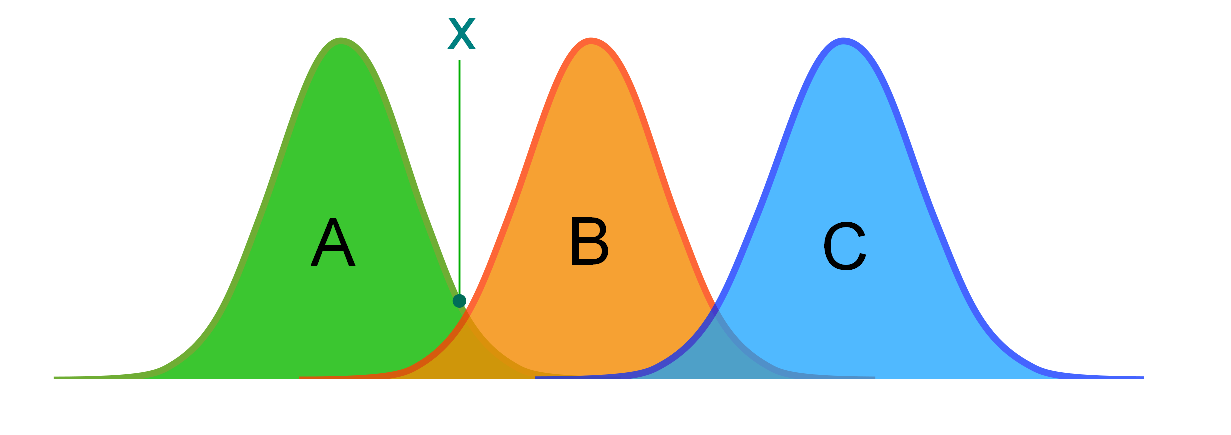
\includegraphics[width=\columnwidth]{figures/toy_example.eps}}
\caption{A toy example showing that the majarity rule (ignoring class
  C entirely) can be sub-optimal. The rare occurences of examples from
  class C in the neighborhood of $x$ provides useful information
  regarding the true label of $x$.}
\label{fig:toy_example}
\end{center}
\vskip -0.2in
\end{figure} 

Our approach is related to work on learning label embeddings~
\cite{Collins2009, Dietterich, Allwien-Schapire, Singer,
  Bengio2010}. The main difference is that our approach is far
simpler, does not require any convex optimizations and can be
seemlessly integrated into the $k$-NN framework. Another related work
is \cite{Bilmes} which introduces a bias term to the likelihood ratio
testing which is justified by the difference between the estimated and
the true class conditional probability.

This paper is organized as follows. In Section~\ref{sec:background},
we describe the framework and the notations. In
Section~\ref{sec:min_kl}, we describe our approach and
justification. In Section~\ref{sec:results}, we present experiments
comparing our approach with the traditional $k$-NN algorithm using
both synthetic data and real-world data. Then, we discuss the results
in Section~\ref{sec:discussion} and conclude the paper in
Section~\ref{sec:conclusion}.

\section{Background}
\label{sec:background}

\newcommand{\X}{\mathcal{X}}
\newcommand{\Y}{\mathcal{Y}}
\newcommand{\trainset}{\mathcal{S}}

Let $\trainset = \{ (x_1,y_1,) \ldots (x_n,y_n)\}$ be a set of
training examples where each instance $x_i$ comes from an example
space $\X$ of which the distance measure is given by
$d(\cdot,\cdot)$. Without loss of generality, we assume that each
label $y_i$ takes on a value from $\Y = \{1,2,\ldots,m\}$.

\newcommand{\nh}{\mathcal{N}}
\newcommand{\Pemp}{\widehat{\mathbf{P}}^x}
\newcommand{\Ptrue}{\mathbf{P}^x}

Let $\nh_k(x)$ denote the neighborhood of size $k$ of an example $x
\in \X$ with respect to the distance measure $d$. The traditional
$k$-NN rule predicts the label of an example $x$ with the majority of
the labels in $\nh_k(x)$. More formally, given $x$ and $\nh_k(x)$, we
can define an empirical distribution $\Pemp$ such that, for each $i \in \Y$, 
\[
\Pemp(i) = \frac{\#\{ \mbox{occurrences of label } i \mbox{ in } \nh_k(x)\}}{k}
\]
The $k$-NN rule predicts the label $\hat{y}$ such that
\[
\hat{y} = \arg\max_{i \in \Y} \: \Pemp(i)
\]

For any example $x \in \X$, we can consider the true class
distribution of $x$, $\Ptrue$ which is given by, for each $i \in \Y$,
\[
\Ptrue(i) = \Pr(Y=i | X=x)
\]
Under certain assumptions, it is shown in \cite{Fix1951} that,
for every class label $i \in \Y$, 
\[
\lim_{\substack{n \to \infty\\k \to \infty\\k/n \to 0}} \Pemp(i) = \Ptrue(i)
\]
Therefore, the majority rule is asymptotically optimal. However, in
the finite sample case, it can be sub-optimal due to the discrepancy
between the empirical distribution $\Pemp$ and the true distribution
$\Ptrue$ as demonstrated by a toy example in Figure~\ref{}

\section{Minimizing KL-Divergence Approach}

\newcommand{\dkl}{D_{\mathrm{KL}}}
\newcommand{\Qemp}{\widehat{\mathbf{Q}}^j}
\newcommand{\Qtrue}{\mathbf{Q}^j}

%%%%%%%%%%%
\iffalse
\[
\Qtrue(i) = \mathbb{E}_{(x,j) \in \trainset} [ \Ptrue(i) ]
\]
\fi
%%%%%%%%%%%

We propose a modification to the $k$-NN rule such that the entire
class distribution $\Pemp$ is taken into account instead of just the
mode of $\Pemp$. Given a training set $\trainset$, we define,
for each class $j$, a prototypical distribution $\Qemp$ such that
\[
\Qemp(i) = \frac{\sum_{(x,j) \in \trainset_j} \Pemp(i)}{|\trainset_j|}
\]
where $\trainset_j = \{ (x,y) \in S | y = j \}$. Essentially, the
prototypical distribution $\Qemp$ is the average class distribution
among the examples from class $j$. It describes how likely is an
example from class $j$ get confused with other classes.

To classify a new example $x$, the empirical class distribution $\Pemp$ is
compared to each prototypical distribution $\Qemp$ for $j \in \Y$ with
respect to a distance measure $g(\cdot ; \cdot)$ and the class label that
minimizes the distance is then predicted. More formally, the predicted
label $\hat{y}$ of an example $x$ is given by
\[
\hat{y} = \arg\min_{j \in \Y} \: g(\Pemp ; \Qemp)
\]

A natural choice for the function $g$ is the KL-divergence function,
which is commonly used for measuring a distance between two
distributions. The KL-divergence $\dkl$ between two distributions
$\mathbf{P}$ and $\mathbf{Q}$ is defined as
\[
\dkl(\mathbf{P} || \mathbf{Q}) = \sum_i \mathbf{P}(i) \log \frac{\mathbf{P}(i)}{\mathbf{Q}(i)}
\]

We show that, when the true class distribution $\Ptrue$ for each
example $x$ of class $j$ in the training set $\trainset$ is identical
to $\Qemp$, the KL-divergence is an optimal measure. The proof is
given by Lemma~\ref{lemma:dkl} and Collorary~\ref{col:min_dkl}. 

\newcommand{\sampleYK}{y^k}
\newcommand{\sampleEmpDist}{\mathbf{P}_{y^k}}
\newcommand{\Q}{\mathbf{Q}}

Let $\sampleYK = [y_1, \ldots, y_k]$ denote a sample of size $k$ drawn IID
from a fixed distribution over $Y$ and let $\sampleEmpDist$ denote the
empirical distribution induced by the sample
$\sampleYK$. Specifically,
\[
\sampleEmpDist(i) = \frac{\#\{ \mbox{occurrences of } i \mbox{ in } y^k\}}{k}
\]

\begin{lemma}
\label{lemma:dkl}
For any distribution $\Q$ and for any sample $\sampleYK$ (not neccessarily
drawn from $\Q$), the likelihood of $\sampleYK$ drawn from $\Q$ is given by
\[
\Q(y^k) = 2^{-k(H(\sampleEmpDist) + \dkl\sampleEmpDist || \Q))}
\]
\end{lemma}
\begin{proof}
  \begin{align*}
    \Q(y^k) 
&= \prod_{l=1}^k \Q(y_l)\\ 
&= \prod_{j \in \Y} Q(j)^{n\sampleEmpDist(j)}\\ 
&= \prod_{j \in \Y} 2^{n\sampleEmpDist(j) \log \Q(j)}\\ 
&= \prod_{j \in \Y} 2^{n(\sampleEmpDist(j) \log \Q(j) - \sampleEmpDist(j) \log \sampleEmpDist(j) + \sampleEmpDist(j) \log \sampleEmpDist(j))}\\ 
&= 2^{k \sum_{j \in \Y} (-\sampleEmpDist(j) \log \frac{\sampleEmpDist(j)}{\Q(j)} + \sampleEmpDist(j) \log \sampleEmpDist(j))}\\ 
&= 2^{k(-\dkl(\sampleEmpDist||\Q) - H(\sampleEmpDist))}\\
  \end{align*}
\end{proof}

\begin{collorary}
\label{col:min_dkl}
Given a set of distributions $\mathcal{Q} = \{\Q_1,\Q_2, \ldots,
\Q_{m}\}$ and a sample $\sampleYK$ drawn from any distribution, the
likelihood of $\sampleYK$ is maximized under $\Q_{i^*}$ if and only if
the KL-divergence from $\sampleEmpDist$ to $\Q_{i^*}$ is minimized.
\[
 i^* = \arg\max_{i \in \Y} \log \Q_i(y^k) = \arg\min_{i \in \Y} \dkl(\sampleEmpDist||\Q_i)
\]
\end{collorary}
\begin{proof}
  Applying Lemma~\ref{lemma:1}, we have
  \begin{align*}
    \Q_i(y^k) &= 2^{-n(H(\sampleEmpDist) + \dkl\sampleEmpDist || \Q_i))}\\
    \log \Q_(y^k) &= -n(H(\sampleEmpDist) + \dkl(\sampleEmpDist || \Q_i))\\
    \arg\max_{i \in \Y} \log \Q(y^k) &= \arg\max_{i \in \Y} - n\dkl(\sampleEmpDist || \Q_i))\\ 
    &= \arg\min_{i \in \Y} \dkl(\sampleEmpDist || \Q_i))\\
  \end{align*}
\end{proof}

As a result, we expect our approach to perform well when 
\[
\frac{\sum_{(x,y) \in \trainset_j} \dkl(\Pemp || \Qemp)}{|\trainset_j|}  \le \epsilon
\]
where $\epsilon$ is small and we expect it to perform optimally when
$\epsilon = 0$. Note that when $\Qemp$ is concentrated exclusively on
class $j$, our approach actually reduces to the majority rule. A
summary of our algorithm is given in Algorithm~\ref{alg:minkl}.

\begin{algorithm}
\caption{The MinKL $k$-NN rule}
\label{alg:minkl}
\begin{algorithmic}[1]
\REQUIRE{A training set $\trainset$ \\ A test example $\tilde{x}$ and its
  neightborhood $\nh_k(\tilde{x})$}
\OUTPUT{Predicted label $\hat{y}$}
\STATE $\widehat{\Q}_i \leftarrow \vec{0} \mbox{ for } i \in \Y$
\FOR{Each example $(x,j) \in \trainset$}
\STATE $\widehat{\Q}_j \leftarrow \widehat{\Q}_j + \Pemp$
\ENDFOR
\STATE $\widehat{\Q}_i \leftarrow \widehat{\Q}_i / |\trainset_i| \mbox{ for } i \in \Y$
\STATE $\hat{y} = \arg\min_{i \in \Y} \dkl(\widehat{\mathbf{P}}^{\tilde{x}} || \Q_i)$
\end{algorithmic}
\end{algorithm}

\section{Experiments}

In this section, we describe experiments we have performed with both
synthetic data and real-world data. Our primary goal is to compare the
classification errors of our proposed algorithm (MinKL) with those of
the traditional $k$-NN rule (Majority) under various conditions.  As
for the real-world data, we performed our experiments on an online
character recognition dataset: uRight and two image-classification
datasets: MNIST, SVHN.

\begin{table}[t]
\caption{A summary of the datasets}
\label{table:datasets}
\vskip 0.15in
\begin{center}
\begin{small}
\begin{sc}
\begin{tabular}{lcccr}
\hline
\abovespace\belowspace
Dataset & No. of classes & validation && epsilon\\
\hline
\abovespace
Synthetic-1   & 10 & 5-fold && \\
Synthetic-2 & 81 & 5-fold && \\
\belowspace
MNIST & 10 & test set provided && \\
SVHN & 10 & test set provided && \\
uRight & 26 & 5-fold && \\
\hline
\end{tabular}
\end{sc}
\end{small}
\end{center}
\vskip -0.1in
\end{table}

\subsection{Synthetic data}
Our synthetic data can be described as follows. Each instance is a
point in a taurus-like $d$-dimensional hypercube $[0,b-1]^d$. There is
a total of $b^d$ classes and the instances of each class are generated
by a normal distribution with mean located at an integer lattice point
of the hypercube and a covariance matrix $\sigma I_d$. Figure~\ref{}
shows a 2-d representation of each class where $b=5, d= 2$ and $\sigma
= 0.5$. We use Manhattan distance as the similarity measure for the
$k$-NN algorithm.

In the first experiment, we generate a dataset, called \textbf{SYN-1},
using $b=10, d=1$ and $\sigma=1.5$. There is a total of 10 classes in
Synthetic-1. In Figure~\ref{} , we show the 5-fold cross validation
error rate of MinKL and Majority using different $n$ and $k$. Using
the optimal $k$ for each $n$, we compare the error rates of MinKL,
Majority and the Bayes optimal classifier at different $n$ in
Figure~\ref{}. 


Next, we generate a more complex dataset, called Synthetic-2, using
$b=3$, $d=4$ and $\sigma=0.4$. This results in a total of $81$ different
classes. Again, in Figure~\ref{}, we show the 5-fold cross validation
error rate of MinKL and Majority using different $n$ and $k$ and
compare the error rate of MinKL, Majority and Bayes optimal at
different $n$ while $k$ is optimized.


\subsection{uRight}
The uRight dataset is our dataset of handwriting trajectories of
English characters. Each example is a sequence of $(x,y)$-coordinates
representing an English letter. We collected this data from 20
different users writing on a touch screen of a mobile phone. There is
a total of about 10000 examples. The similarity between any two
examples is measured by the dynamic time wraping distance between
them~\cite{}.

We performed the analysis for each user. The 5-fold cross validation
results are shown in Figure~\ref{}.

We also show some of the examples that are misclassified by the
Majority but not the MinKL in Firgure~\ref{}.


\subsection{MNIST}
Each instance in the MNIST dataset~\cite{} is a 28x28 grayscale image. There
are 60000 training examples and 10000 testing examples. The dataset
has been widely used as a benchmark for classification algorithms. We
prepropress the data by deskewing, resampling the images down to
14x14 pixels, and applying PCA. We transform each image into a feature
vector which is the top 100 PCA components. We use Euclidean distance
as the similarity measure for the $k$-NN algorithm.

The results are summarized in Figure~\ref{}. 

\subsection{SVHN}
The SVHN dataset~\cite{} contains images of digits taken from the Google
street view data. It is considered a harder dataset than the
MNIST. Each instance in the SVHN dataset is a 32x32 RGB image
patch. There are 73257 training examples and 26032 testing
examples. We preprocess the images by deskewing and then extract the
HOG features~\cite{} from the images. We use Manhattan distance as the
similarity measure of the $k$-NN algorithm.

The results are summarized in Figure~\ref{}.



\section{Discussion}

From the experiments, we noticed that MinKL approach performs
significantly better than Majority in the small sample situation. As
the number of training examples increases, the gap of the performance
of the two approaches decreases. We anticipated this since the
Majority vote rule is proven to be optimal asymptotically. In some
applications, it is crucial to perform well even when there are only a
few training examples. This is where we believe that our approach has
advantage over the majority vote.

In analysis, we have shown that our approach is optimal when the data
is generated under certain assumptions. For real-world data,
such assumptions may or may not hold. Nonetheless, we can see some
improvements in our experiments. We suspect that our approach will be
more beneficial to problems with a large number of classes and the
confusions between classes are non-uniform. 

In a sense, our approach naturally incoporates the infomation from the
label space into the classification. The label space information is
encoded into the prototypical neighborhood distribution. The
performance of our approach depends on how
different the prototypical neighborhood distributions of different
classes are. If the prototypical distributions are similar, then our
approach will suffer. A workaround is to have multiple prototypical
distributions per class. 

Our approach does not have a consistency gaurantee. It is
possible that our approach will be sub-optimal when the number of
training examples goes to infinity because the prototypical
distribution model is incorrect or insufficent. We do not worry
about this problem that much since we see our approach being used
in a small sample scenario.

In practice, other divergences might work better than the KL
divergence. The KL divergence is considered a special case of a
more general divergence function called Alpha-divergence which is
given by
\[
D^{(\alpha)}_A (p||q) = \frac{1}{\alpha(\alpha - 1)}\left( \sum_1^n
  p^{\alpha}_i q^{1-\alpha}_i - 1\right), \; \alpha \in \mathrm{R} \ \{0,1\}
\]
The KL-divergence can be expressed as $D_{KL} (p || q) = \lim_{\alpha
\rightarrow 1} D^{(\alpha)}_A (p || q)$. 
For uRight dataset, we were able to obtain better classification
accuracy by using Alpha-divergence with $\alpha = 2$.

Our approach can be applied to other classification algorithms as
well. The $k$-NN algorithm is very computational expensive when
classifying a new example. For some applications, it is
important to be able to classify new examples quickly. A simple
modification to the $k$-NN algorithm is to keep a small number of
representatives for each class and discard the rest. This algorithm is
called the $k$ nearest-centroid algorithm ($k$-NC) where only the
$k$-centroids are kept as the class representatives. In the $k$-NC,
the class posterior distribution can be estimating by
\[
p(y|x) = \frac{e^{d(x,C(y))}}{\sum_j e^{d(x, C(j))} }
\]
We can apply the MinKL technique to the class posterior computed this
way. In Figure~\ref{}, we compare the accuracy of the $k$-NC algorithm
with MinKL and Maximum (equavalent to Majority in the $k$-NN).

\section{Conclusions}

We suggest a simple modification to the $k$-NN algorithm.

\bibliography{example_paper}
\bibliographystyle{icml2014}

\end{document} 


% This document was modified from the file originally made available by
% Pat Langley and Andrea Danyluk for ICML-2K. This version was
% created by Lise Getoor and Tobias Scheffer, it was slightly modified  
% from the 2010 version by Thorsten Joachims & Johannes Fuernkranz, 
% slightly modified from the 2009 version by Kiri Wagstaff and 
% Sam Roweis's 2008 version, which is slightly modified from 
% Prasad Tadepalli's 2007 version which is a lightly 
% changed version of the previous year's version by Andrew Moore, 
% which was in turn edited from those of Kristian Kersting and 
% Codrina Lauth. Alex Smola contributed to the algorithmic style files.  
